\section{312 --- Burst Balloons}
Given $ n $ balloons, indexed from 0 to $ n-1 $. Each balloon is painted with a number on it represented by array nums. You are asked to burst all the balloons. If the you burst balloon i you will get nums[left] * nums[i] * nums[right] coins. Here left and right are adjacent indices of i. After the burst, the left and right then becomes adjacent.
\par
Find the maximum coins you can collect by bursting the balloons wisely.

\paragraph{Note:}

\begin{itemize}
\item You may imagine $A[-1] = A[n] = 1$. They are not real therefore you can not burst them.
$0 \leq n \leq 500$, $0 \leq A[i] \leq 100$
\end{itemize}

\paragraph{Example:}

\begin{flushleft}
\textbf{Input}: $[3,1,5,8]$
\\
\textbf{Output}: 167 
\\
\textbf{Explanation}: 
\begin{figure}[H]
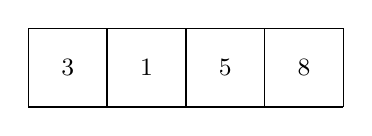
\begin{tikzpicture}
\draw[line width=0.5pt] (0,0) grid (4,1);
\node at (0.5,0.5) {{\small 3}};
\node at (1.5,0.5) {{\small 1}};
\node at (2.5,0.5) {{\small 5}};
\node at (3.5,0.5) {{\small 8}};
\end{tikzpicture}
\end{figure}
Burst ballon with number 1, get coins $=3\times 1\times5  $
\begin{figure}[H]
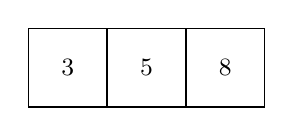
\begin{tikzpicture}
\draw[line width=0.5pt] (0,0) grid (3,1);
\node at (0.5,0.5) {{\small 3}};
\node at (1.5,0.5) {{\small 5}};
\node at (2.5,0.5) {{\small 8}};
\end{tikzpicture}
\end{figure}
Burst ballon with number 5, get coins $=3\times 5\times 8  $
\begin{figure}[H]
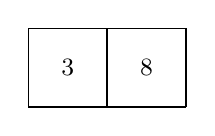
\begin{tikzpicture}
\draw[line width=0.5pt] (0,0) grid (2,1);
\node at (0.5,0.5) {{\small 3}};
\node at (1.5,0.5) {{\small 8}};
\end{tikzpicture}
\end{figure}
Burst ballon with number 3, get coins $=1\times 3\times  8  $
\begin{figure}[H]
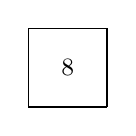
\begin{tikzpicture}
\draw[line width=0.5pt] (0,0) grid (1,1);
\node at (0.5,0.5) {{\small 8}};
\end{tikzpicture}
\end{figure}
Finally burst ballon with number 8, get coins $=1\times  8\times 1  $
\\
The total coins = $ 3\times 1\times5 + 3\times 5\times 8 +1\times 3\times  8 +1\times  8\times 1 = 167 $
\end{flushleft}
\subsection{Dynamic Programming}
\begin{itemize}
\item 这是一个2D dynamic programming。因此定义\texttt{DP} array $F[i][j]$表示the maximum coins by bursting all ballons from $ A[i] $ to $ A[j] $。
\item 这里有个trick的点,即$F[i][j]$是burst all ballons from $ A[i] $ to $ A[j] $,这意味着在$ [i,j] $中的某个index $ k $,如果计算出$ F[i][k-1] $和 $ F[k+1][j] $,也就意味着 $ A[i] $和$ A[j] $就不再和$ A[k] $相邻了。这时候$ A[k] $的左右边两边的ballon分别是$ A[i-1] $和$ A[j+1] $了。
\item 基于上述分析,对于$ [i,j] $中的某个index $ k $,即$ i\leq k\leq j $,如果选择burst $A[k]$,那么所获得的maximum coins为$F[i][k-1] + F[k+1][j] + A[i-1]\times A[k]\times A[j+1]$。所以$ F][j] = \max(\underbrace{F[i][k-1] + F[k+1][j] + A[i-1]\times A[k]\times A[j+1]}_{i\leq k\leq j}$
\item 由于$i\leq k\leq j$,那么当$k=i$或者$k=j$时,会出现$ F[i][i-1] $和$ F[j+1][j] $,这个是$F$的左下三角,而$ F $的更新都在右上三角,初始化时都设为零,因此不会有问题。
\item 另外,当只有一个元素的时候,$ F $的递推会越界,为了解决这个问题,在$ A $的前后分别加上1。然后$F$的dimension为$ (L+2)\times(L+2) $。最后返回$F[1][L]$ ($ L $ is the size of $ A $)。
\item 在进行$ F $递推时,最外层循环当前更新的长度$ \ell $,从1到$ L $,而内层循环的$l$则从1开始,因为我们已经插入了1在最前面。同样$ l $循环到$l+\ell-1 = L$为止,因为也插入了1在最后面。
\end{itemize}
\setcounter{lstlisting}{0}
\begin{lstlisting}[style=customc, caption={Dynamic Programming}]
int maxCoins( vector<int>& nums )
{
    int sz = static_cast<int>( nums.size() );

    //Add 1 to begin and end of A
    vector<int> A( nums.size() + 2, 1 );

    auto it = A.begin();
    ++it;

    copy( nums.begin(), nums.end(), it );

    vector<vector<int>> F( sz + 2, vector<int>( sz + 2, 0 ) );

    //Filling the up right triangle of F
    for( int l = 1; l <= sz; ++l )
    {
        for( int x = 1; x + l - 1 <= sz; ++x )
        {
            int y = x + l - 1;

            for( int k = x; k <= y; ++k )
            {
                //All ballons from A[x] to A[y] are bursted
                //A[k] is adjacent to A[x-1] and A[y+1]
                int coins = A[k] * A[x - 1] * A[y + 1];
                //burst all ballons from A[x] to A[k-1]
                coins += F[x][k - 1];
                //burst all ballons from A[k+1] to A[y]
                coins += F[k + 1][y];

                F[x][y] = ( max )( F[x][y], coins );
            }
        }
    }

    //F[1][sz] is the result for burst
    //all ballons from A[0] to A[sz-1]
    return F[1][sz];
}

\end{lstlisting}

\paragraph{Related Problems}
\begin{itemize}
\item \textbf{1000. Minimum Cost to Merge Stones}
\end{itemize}